\section{Procedimentos}
\label{sec:procedimentos}

Neste trabalho foi proposto um processo que deve guiar o desenvolvimento durante a execução deste estudo de caso. A partir da revisão da literatura descrita em \ref{ch:revisao}, procurou-se compreender as atividades envolvidas na experimentação continua e encontrar modelos ou processos já existentes na literatura. 

Em seguida, buscou se analisar o processo atual da empresa, compreendendo as atividades já existentes e realizadas pelos desenvolvedores do produto para posterior definição de atividades que viabilizariam a execução de experimentos controlados. Esta formalização se baseou principalmente no modelo \textit{Combined Process for Experimentation}, proposto por \citeonline{erthal_characterization_2023} e já apresentado na Figura \ref{fig:erthal-process}.

Feita essa formalização, através dos insumos encontrados na literatura, foi proposto um novo processo, visando a introdução de práticas de experimentação contínua e que servirá de objeto de estudo desta monografia. A versão inicial, que ilustra o processo de desenvolvimento atualmente utilizado pela empresa, é apresentado na Figura \ref{fig:processo-atual}. Já o processo proposto neste trabalho, adaptado a partir do atual, é apresentada na Figura \ref{fig:processo-novo}, onde os itens destacados de vermelho são as novas atividades e artefatos, trazendo o fluxo que deve ser seguido nesta investigação.

Para a coleta de dados referentes aos resultados das atividades realizadas e como o processo proposto se desempenhou, serão realizados questionários, que devem ser respondidos pelos colaboradores participantes. Já os dados de segunda ordem, ou seja, aqueles coletados por meio de observações, serão as métricas e medidas de qualidade em uso definidas durante a ideação da hipótese a ser testada pelo experimento que será realizado.


\begin{figure}
    \centering
    \caption{Modelo do Fluxo de Atividades Atual do Produto Investigado}
    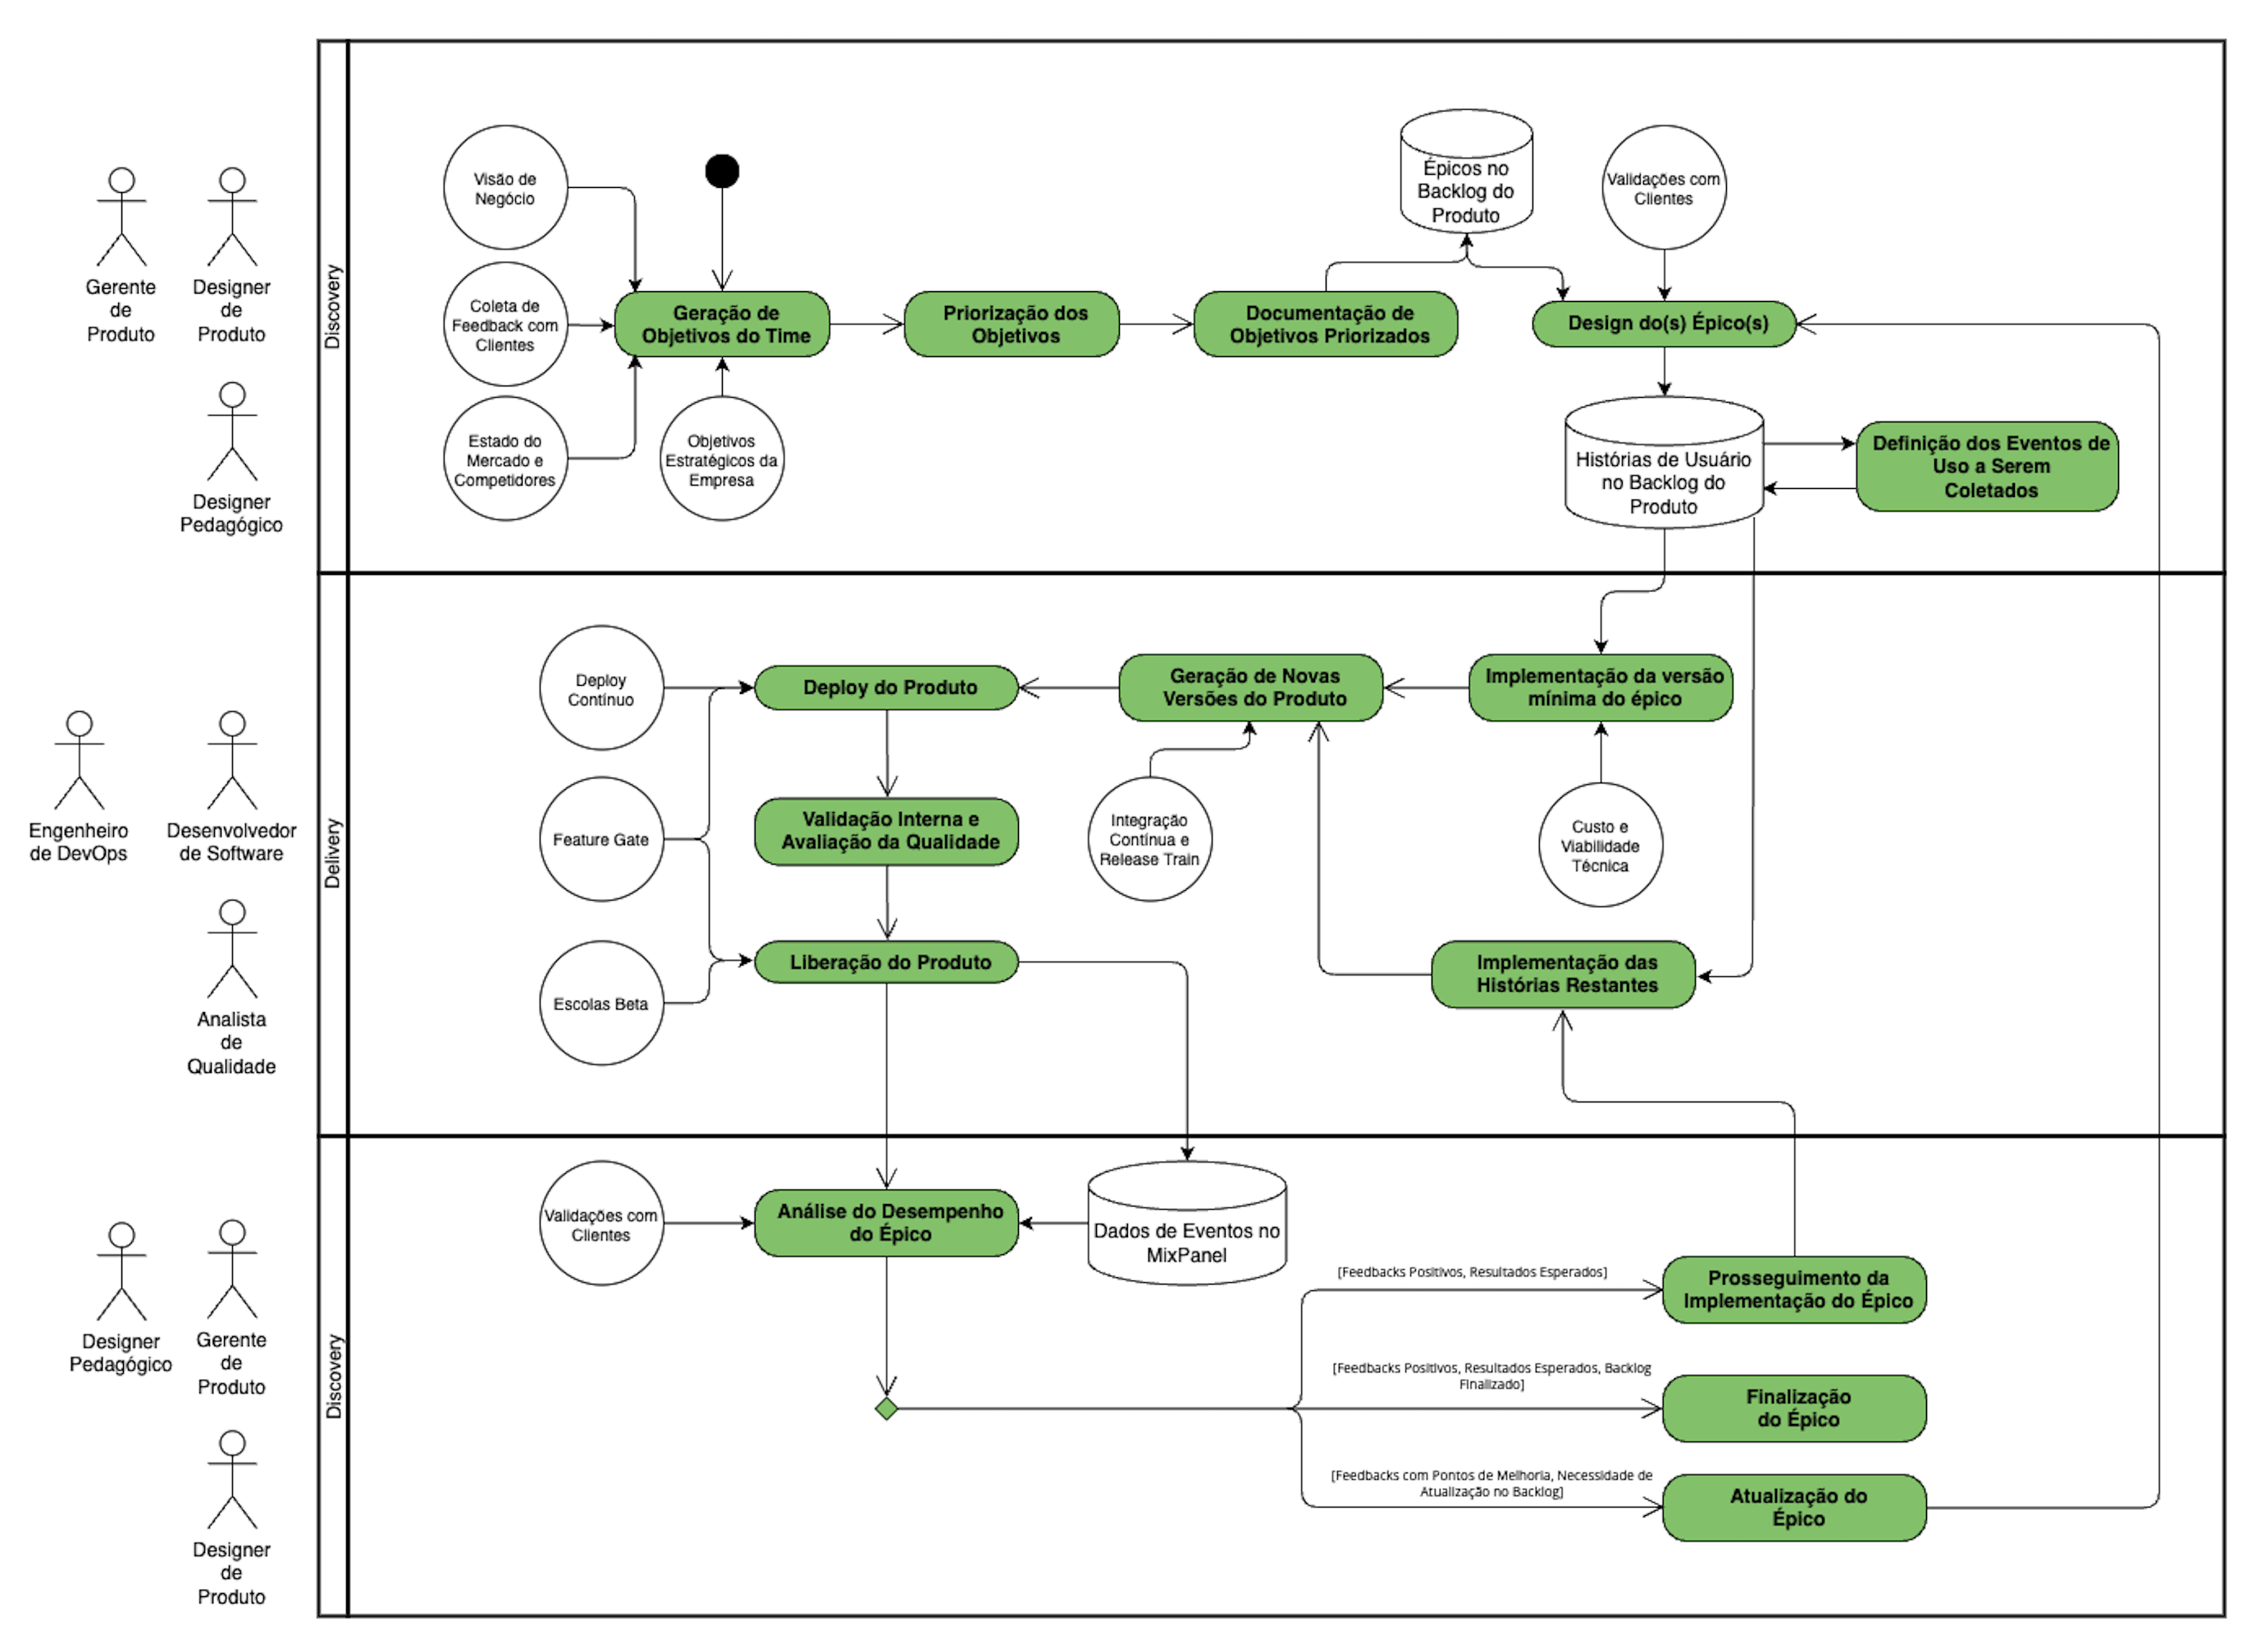
\includegraphics[width=1\linewidth]{figuras/processo-atual.png}
    \begin{center}
        \text{Fonte: Autor}
    \end{center}
    \label{fig:processo-atual}
\end{figure}

\begin{figure}
    \centering
    \caption{Modelo Proposto Para Implementação da Experimentação Contínua}
    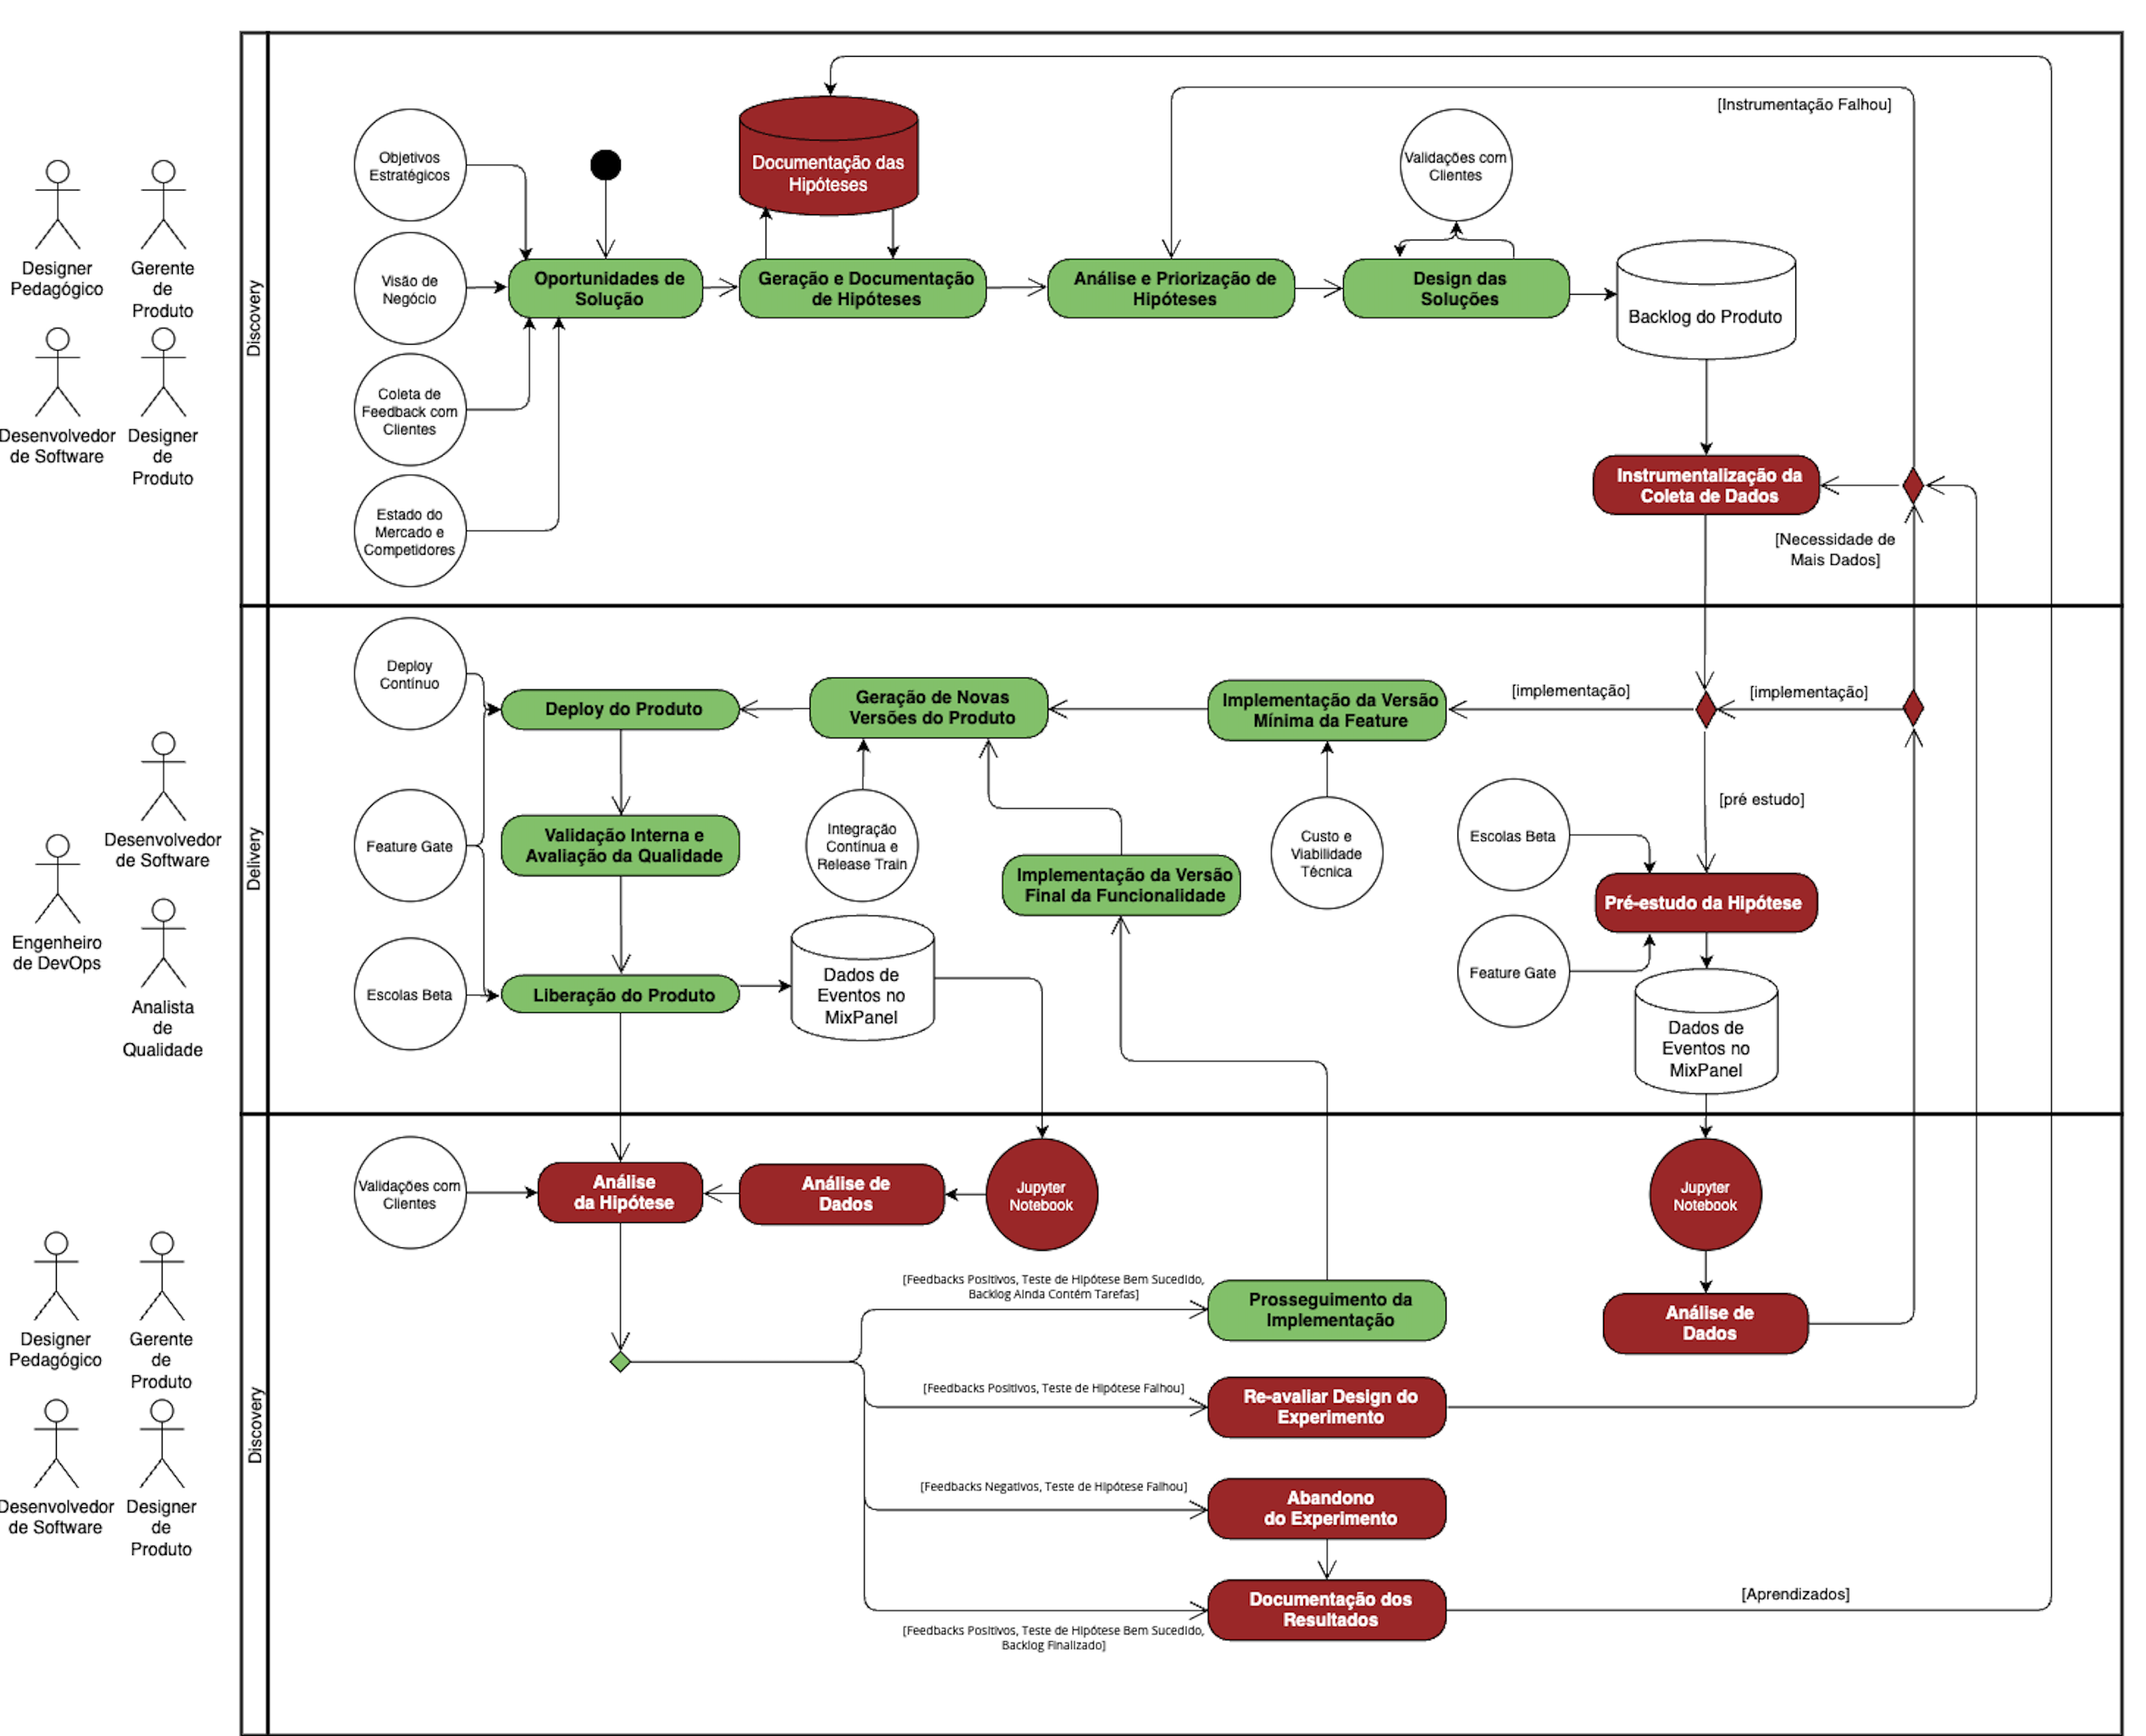
\includegraphics[width=1\linewidth]{figuras/processo-novo.png}
    \begin{center}
        \text{Fonte: Autor}
    \end{center}
    \label{fig:processo-novo}
\end{figure}


\subsection{Processo Proposto}
\label{subsec:fluxo}

Aqui serão descritas as atividades, fases, papeis e artefatos do processo proposto. Determinadas atividades do processo são iterativas e devem/podem ser realizadas novamente caso necessário. Abaixo são descritas as atividades a serem realizadas, conforme apresentado na Figura \ref{fig:processo-novo}.

\begin{itemize}
    \item \textbf{Documentação de Hipóteses:} Serão realizadas as atividades da Engenharia de Hipóteses, quer sejam: gerar; documentar; analisar e priorizar as suposições do time. O objetivo é formalizar as suposições em hipóteses para realização de testes estatísticos;
    
    \item \textbf{\textit{Design} do Experimento:} Serão criados os protótipos da hipótese selecionada para desenvolvimento, como já acontece hoje com as funcionalidades da empresa. A diferença é que também serão elencadas métricas do comportamento em uso que devem ser coletadas para avaliação da funcionalidade.

    \item \textbf{Instrumentalização da Coleta de Dados:} O ambiente de coleta de métricas e medidas será preparado; Antes do desenvolvimento efetivo da versão de tratamento, os eventos de uso necessários serão adicionados no código-fonte, separando as populações através de \textit{feature flags}.

    \item \textbf{Pré Estudo da Hipótese:} Antes da implementação e com a coleta de dados instrumentalizada, será feito um Teste A/A: ambas as populações serão expostas à versão de controle. O propósito é que o \textit{design} do experimento seja avaliado e a equipe retorne ao processo de instrumentalização ou análise da hipótese caso seja necessário.

    \item \textbf{Desenvolvimento do Tratamento:} A nova versão deve ser desenvolvida conforme planejado e liberada para os usuários selecionados.

    \item \textbf{Análise de Dados:} A partir das métricas coletadas serão realizados testes estatísticos de hipótese que devem ditar a implantação ou abandono da hipótese testada.

    \item \textbf{Coleta de Opinião:} Após a tomada de decisão referente ao experimento, será coletada a opinião dos colaboradores envolvidos referente ao desempenho do processo empregado.
\end{itemize}


